\section{Analiza rezultatov}\label{sec:zakljucek}

Ob pregledu rezultatov in napak, ugotovimo, da na koncu imamo napako. To je lahko iz raznih razlogov, naprimer da nihanje motorja, ki je poganjalo vzmet ni bilo zares sinusno, da ima motor sam napako, med zapisano frekvenco in dejansko frekvenco in podobno. Največja napaka je pri maksimalni meritvi zato, ker je odklon bil tako velik, da več ni bil na merilni lestvici, ter smo ga le aproksimirali na 180 deg.

%%%%%%%%%%%%%%%%%%%%%%%%%%%%%%%%%%%%%%%%%%%%%%%%%%%%%%%%%%
%\makebox[0pt][l]{\begin{minipage}{\textwidth}\centering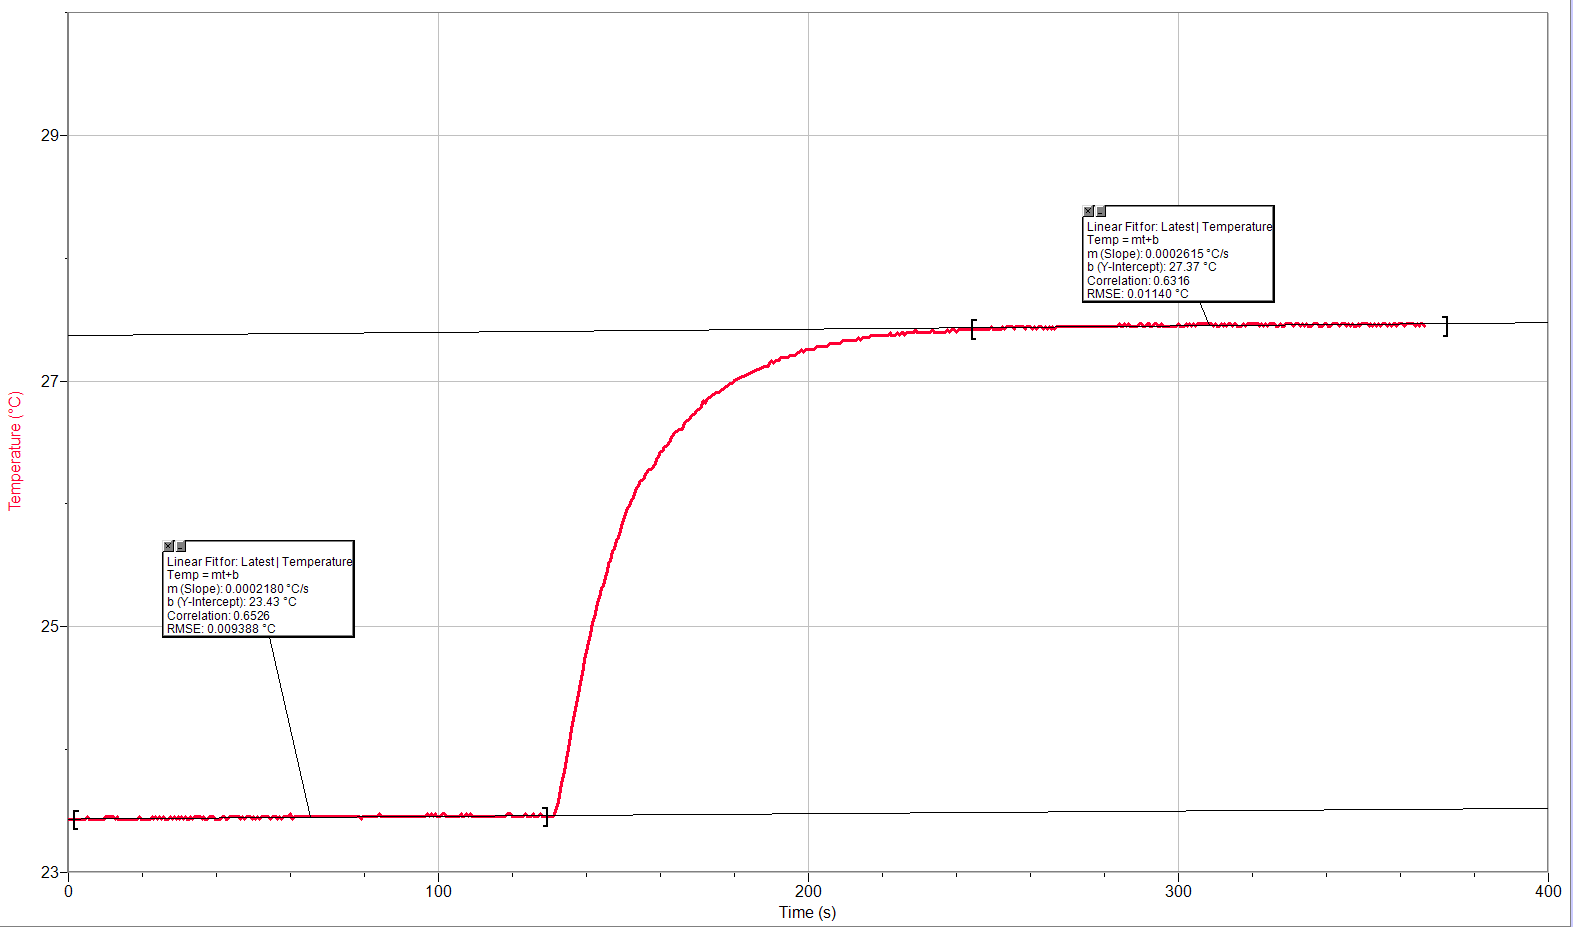
\includegraphics[width=0.8\textwidth]{slike/232.png}\captionof{figure}{Graf meritev masa 1}\end{minipage}}

%\makebox[0pt][l]{\begin{minipage}{\textwidth}\centering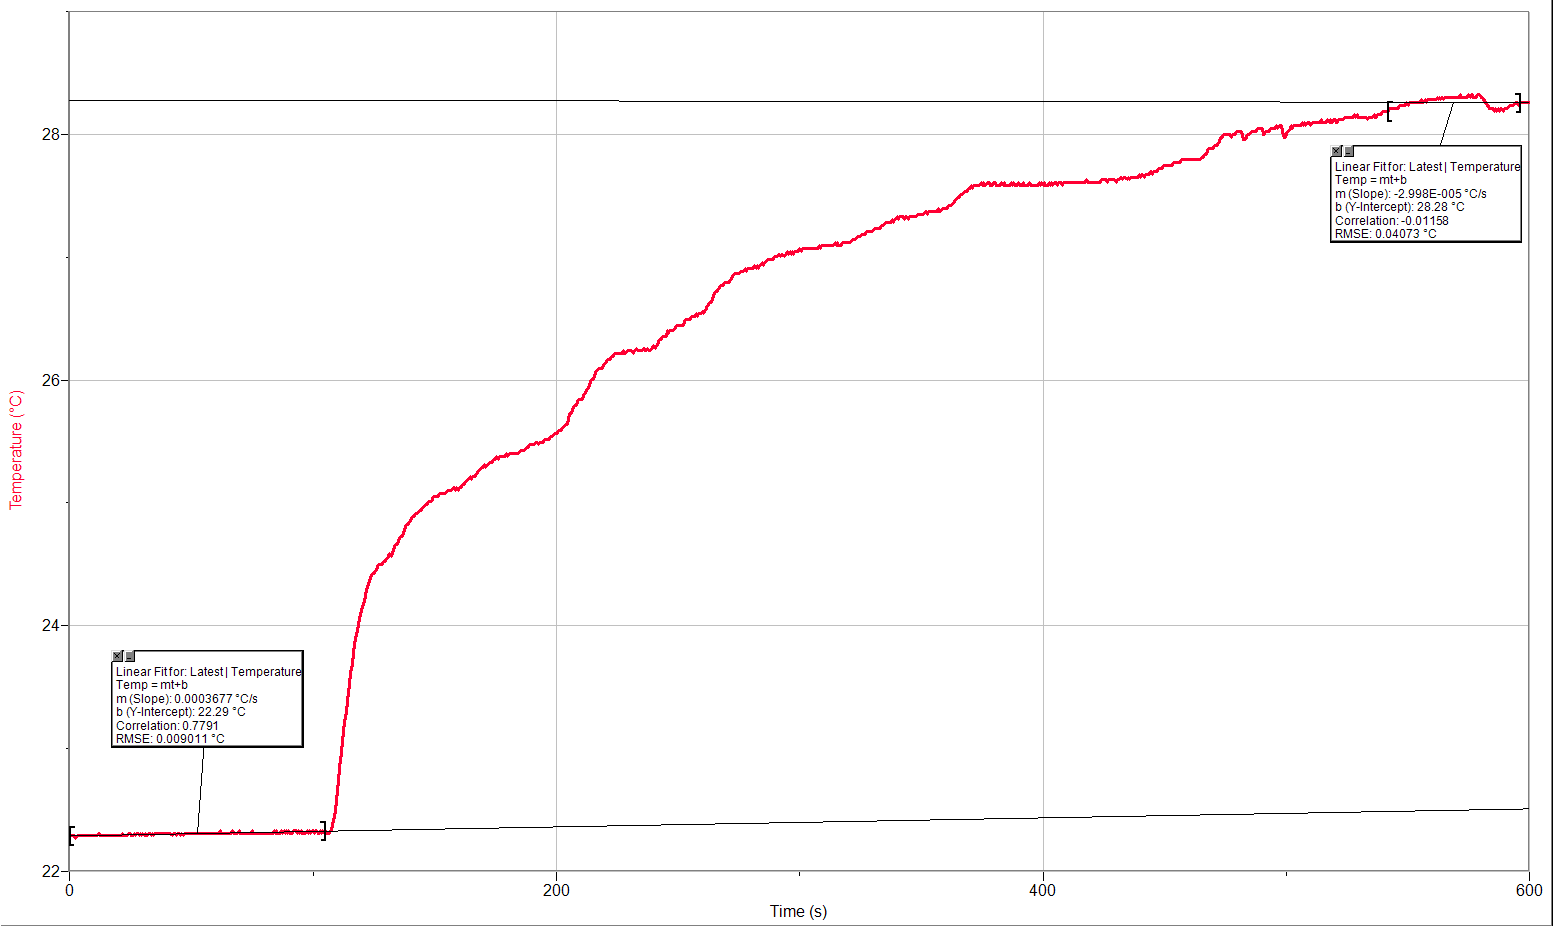
\includegraphics[width=0.8\textwidth]{slike/680.png}\captionof{figure}{Graf meritev masa 2}\end{minipage}}

%\makebox[0pt][l]{\begin{minipage}{\textwidth}\centering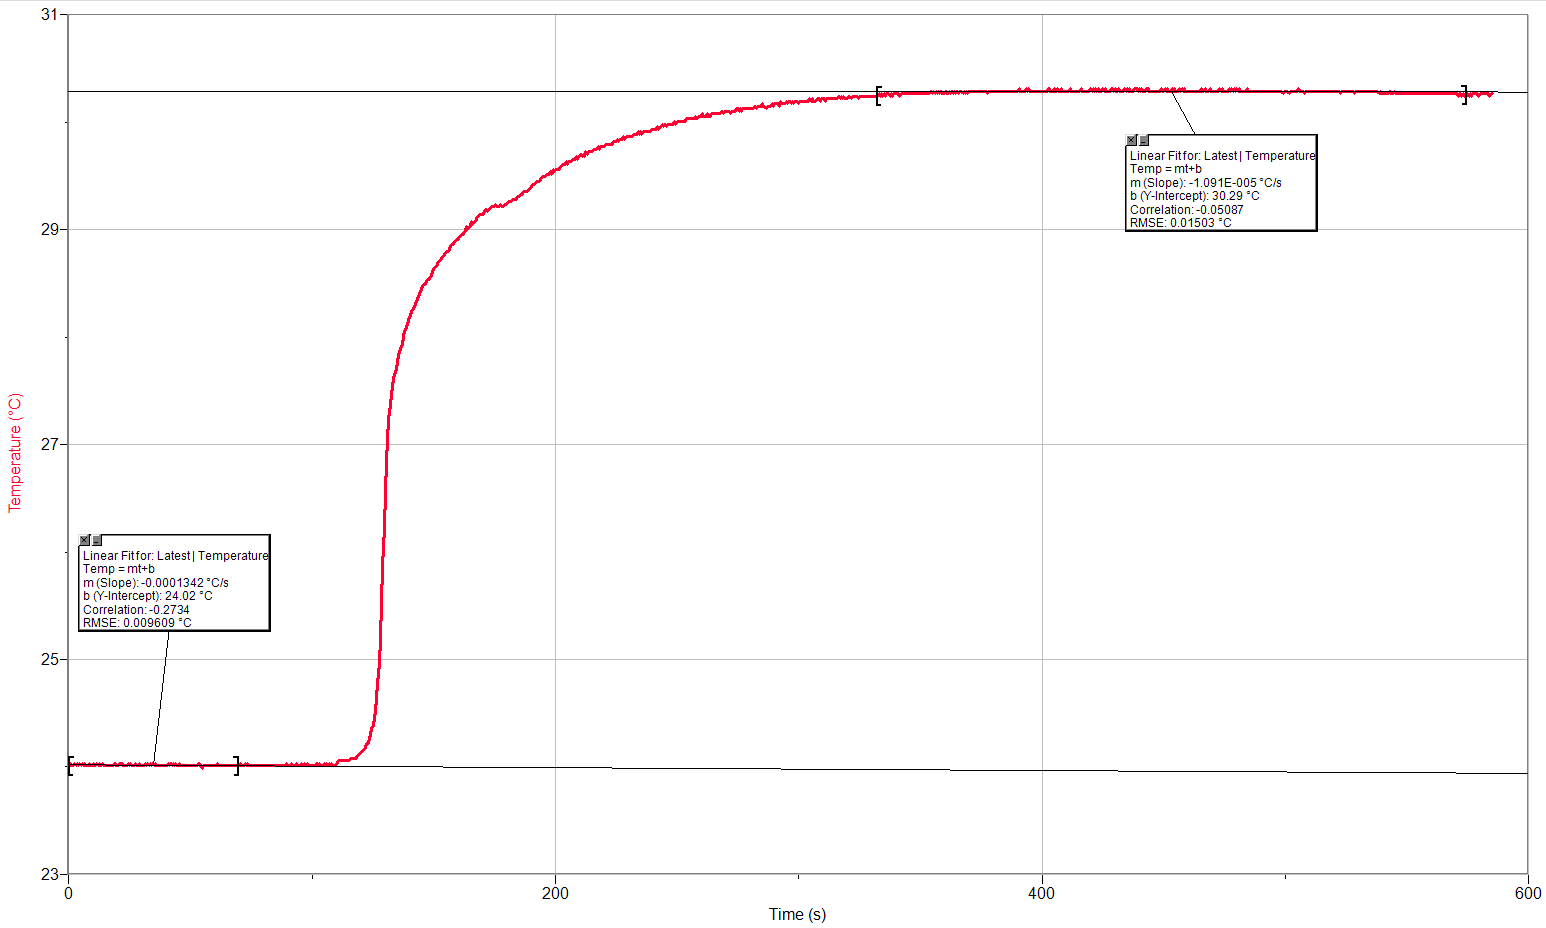
\includegraphics[width=0.8\textwidth]{slike/762.png}\captionof{figure}{Graf meritev masa 3}\end{minipage}}
%%%%%%%%%%%%%%%%%%%%%%%%%%%%%%%%%%%%%%%%%%%%%%%%%%%%%%%%%%